\chapter{Developer documentation}
\label{ch:impl}

This chapter gives the very details of involved technologies, development environment, analysis, implementations and considerations.

\section{Environment Requirements}
The application is supported to be ran and developed both locally and with dedicated cloud application: 
\begin{enumerate}
    \item Possible toolkit for Local environment
        \begin{itemize}
            \item Eclipse with Spring Tools and CAP extensions
            \item Visual Studio Code with SAP CAP extensions
        \end{itemize}
    \item Possible toolkit for Cloud environment
        \begin{itemize}
            \item SAP Business Application Studio with Full-Stack Development dev-space (recommanded, used in this thesis)
        \end{itemize}
\end{enumerate}

For local development, up to date Java JDK, node.js and CAP extensions are hard requirements. The specific set up can be find \hyperlink{https://developers.sap.com/tutorials/btp-app-prepare-dev-environment-cap.html}{here}.

This thesis used SAP Business Application Studio (BAS) as development tool, which is ready for use. 

A snapshot of versions at the time of development:

\lstset{caption={Version check}, label=src:bash}
\begin{lstlisting}[language={bash}]
> java --version
# openjdk 17.0.4.1 2022-08-12 LTS
# OpenJDK Runtime Environment SapMachine (build 17.0.4.1+1-LTS)
# OpenJDK 64-Bit Server VM SapMachine (build 17.0.4.1+1-LTS, mixed mode, sharing)
> cds version
# @sap/cds: 7.2.1
# @sap/cds-compiler: 4.0.2
# @sap/cds-dk: 7.2.0
# @sap/cds-dk (global): 7.2.0
# @sap/cds-fiori: 1.1.0
# @sap/cds-foss: 4.0.2
# @sap/cds-mtxs: 1.11.0
# @sap/eslint-plugin-cds: 2.6.3
# Node.js: v18.14.2

\end{lstlisting}


\section{Run}
The following commands can be used to run the application for testing.

\lstset{caption={Run commands}, label=src:bash}
\begin{lstlisting}[language={bash}]
cds watch # This ... explain!!
\end{lstlisting}
\begin{lstlisting}[language={bash}]
mvn clean install
mvn spring-boot:run
\end{lstlisting}


\section{Analysis and Design}
\subsection{User Story}
\subsection{User Cases}
\subsection{User Diagrams}

\begin{figure}[H]
	\centering
	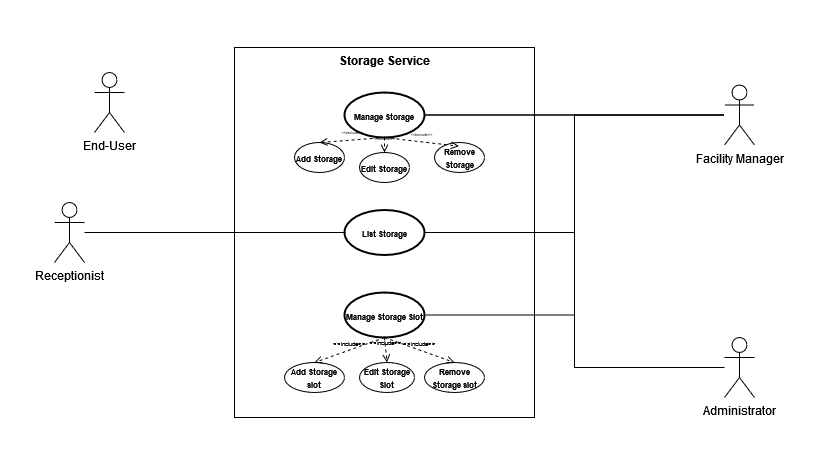
\includegraphics[height=250px]{images/User_Diagram-StorageService.png}
	\caption{Storage Service}
	\label{fig:service-1}
\end{figure}
\section{Application Structure}

The application is developed under the guidence of CAP and is a multi-tenant application. i.e. all three essential parts of the application, front-end, back-end and database are being developed at the same place/project, as a plugged in service, deployed at the same time and interacting with each other on the run time.

\subsection{Overview}
\subsection{Project Structure}
\section{Data Model}
Since Digital Lab provides more then one solutions and to ensure the maximum reuse of models, data model is seperated into 2 parts: solution specific data models and common data models.
\subsection{Specification}
\subsubsection{Solution specific data model}
picture
\subsubsection{General common data model}
picture
\subsection{Implementation}
All data models are modeled by CDS' definition language. Single entities are put into their own \textit{EntityName.cds} files. The main goal is to model out the exact relationships as illustrate in the specification section.

Here list the structure of folders:
\lstset{caption={Structure of folders - data model}, label=src:bash}
\begin{lstlisting}[language={bash}]
root/
    |- db/
        |- data
        |- model
            |- packagehandling 
                |- *.cds # Definition of solution specific data model
            |- common
                |- *.cds # Definition of common data model
\end{lstlisting}

The solution-specific and common data models are also seperated in the sense of names spaces by define the following accordingly at the top of the entities definitions.

\lstset{caption={cds namespaces for data model}, label=src:cds}
\begin{lstlisting}[language={c++}]
namespace com.sap.internal.digitallab.packagehandling.common; // namespace for reusful 
namespace com.sap.internal.digitallab.packagehandling.core; // namespace for solution-specific
\end{lstlisting}

To optimize and standardize the outcome, common \textbf{aspects} (\textit{cuid, managed, User, CodeList}) from \textit{@sap/cds/common} are used in the definition. It can be seen as "extend" in the object-orient way, or more speificly "interface" in Java. Aspects are defined in a similiar way as entities, consists of fields/properties. Entities can "implement" zero to more aspects, "inheriting" aspect's properties and "extend" with its own properties. 

\begin{definition}
    \textbf{CDS's aspects} allow to flexibly extend definitions by new elements as well as overriding properties and annotations. They're based on a mixin approach as known from Aspect-oriented Programming methods.
\end{definition}

Here records the common aspects used by this thesis. \textit{managed} comes with 4 elements: created, created, changed, changed, and automatically updates them. \textit{cuid} automatically assigns UUID primary key to entity. \textit{CodeList} provides a out of box way of implementing enumeration like data structures and supports automatic localization.

\lstset{caption={Aspect managed from @sap/cds/common}, label=src:bash}
\begin{lstlisting}[language={c++}]
aspect managed {
  createdAt  : Timestamp @cds.on.insert : $now;
  createdBy  : User      @cds.on.insert : $user;
  modifiedAt : Timestamp @cds.on.insert : $now  @cds.on.update : $now;
  modifiedBy : User      @cds.on.insert : $user @cds.on.update : $user;
}
\end{lstlisting}

\lstset{caption={Aspect cuid from @sap/cds/common}, label=src:bash}
\begin{lstlisting}[language={c++}]
aspect cuid {
  key ID : UUID; //> automatically filled in
}
\end{lstlisting}

\lstset{caption={Aspect CodeList from @sap/cds/common}, label=src:bash}
\begin{lstlisting}[language={c++}]
aspect CodeList @(
    cds.autoexpose,
    cds.persistence.skip : 'if-unused'
) {
    name  : localized String(255)  @title : '{i18n>Name}';
    descr : localized String(1000) @title : '{i18n>Description}';
}
\end{lstlisting}

Below captures two examples from the thesis on usage of aspects coupled with the SQL DDL corresponding to the cds definition.
\lstset{caption={managed, cuid delivery company entity and corresponding SQL DDL}, label=src:sql}
\begin{lstlisting}[language={sql}]
entity DeliveryCompany : cuid, managed {
    name     : String(255) not null;
    logo     : String(255)  @Core.IsURL  @Core.IsMediaType;
    packages : Association to many Package
                   on packages.deliveryCompany = $self;
}

CREATE TABLE com_sap_internal_digitallab_packagehandling_core_DeliveryCompany (
  ID NVARCHAR(36) NOT NULL,
  createdAt TIMESTAMP_TEXT,
  createdBy NVARCHAR(255),
  modifiedAt TIMESTAMP_TEXT,
  modifiedBy NVARCHAR(255),
  name NVARCHAR(255) NOT NULL,
  logo NVARCHAR(255),
  PRIMARY KEY(ID)
);
\end{lstlisting}

\lstset{caption={codelist package type entity and corresponding SQL DDL}, label=src:sql}
\begin{lstlisting}[language={sql}]
entity PackageType : sap.common.CodeList {
    key code : String(255) not null;
}

CREATE TABLE com_sap_internal_digitallab_packagehandling_core_PackageType (
  name NVARCHAR(255),
  descr NVARCHAR(1000),
  code NVARCHAR(255) NOT NULL,
  PRIMARY KEY(code)
);
\end{lstlisting}
\section{Security}
The application is defined and developed for internal use of company, that is, can be accessed only from SAP devices. The application uses XSA Security and Authentication Service (XSUAA) as for Authentication. Authorization of the application is enforced in the sense of roles' accessibility to the specific services. Four roles are defined, namely Administrator, Facility Manager, Receptionist and End-User. The assignment of roles is done centrally on the Business Technology Platform (BTP), some mock users are also defined for the local development environment.


\subsection{Roles Specification}
All role-specific are set up in the file \textit{root/xs-security.json}. The according restriction on services are defined in \textit{root/srv/services/*-auth.cds} files. As illustrated below.

\lstset{caption={File locations - Security}, label=src:bash}
\begin{lstlisting}[language={bash}]
root/
    |- srv/
        |- src
        |- gen
        |- services
            |- ServiceName 
                |- *.cds # Definition of service
                |- *-auth.cds # Access restriction on roles.
    |- xs-security.json # list of roles
\end{lstlisting}

The access rules of the 4 roles are listed below:

\begin{table}[H]
    \centering
    \begin{tabular}{|c|c|c|c|c|} \hline 
         &  End-User&  Facility Manager&  Administrator&  Receptionist \\ \hline 
         Manage Storage& No  & Yes & Yes & No  \\ \hline 
         Manage Delivery Companies& No & Yes & Yes & No  \\ \hline 
         Manage Packages& No & Yes & Yes & Yes \\ \hline 
         Package Pickup& Yes & Yes & Yes & Yes  \\ \hline 
         Package Registration& No & Yes & Yes & Yes \\ \hline 
         My History& No & Yes & Yes & No \\ \hline
    \end{tabular}
    \caption{Roles Access Rules}
    \label{tab:Access Rule}
\end{table}

\subsection{Mock Users}
To support local development and testing, 4 mock users are defined under \textit{application.yaml}, which will be used in the default spring boot run-time.

Here pasted an example of mock user.

\lstset{caption={Mock Users - Security}, label=src:yaml}
\begin{lstlisting}[language={bash}]
security:
    authentication.normalize-provider-tenant: true
    mock.users:
        admin:
            password: admin
            roles:  
                - Administrator 
        user:
            password: user
                - User
        manager:
            password: manager
            roles:
                - FacilityManager
\end{lstlisting}

\section{UI}
The application utilized UI5 Fiori elements. Every UI related modules are packed under \textit{root/app} folder. In short, Fiori elements are assembled into pages using cds annotations on the exposed services. App router is added to direct urls throughout backend OData services and frontend Fiori web application. End-points are defined again inside \textit{application.yaml}.

\subsection{Folder Structure}
\subsection{Implementation}

\section{Services}
\subsection{Specification}
\subsection{Implementation}

\section{Testing}
\section{Deployment}

\section{Data Model}

\section{Technologies and Terms}
